\documentclass[ManualeUtente]{subfiles}

\begin{document}
	
	\chapter{Admin}
	After logging in as an admin user, you will see this screen:
	\begin{figure}[H]
		\centering
		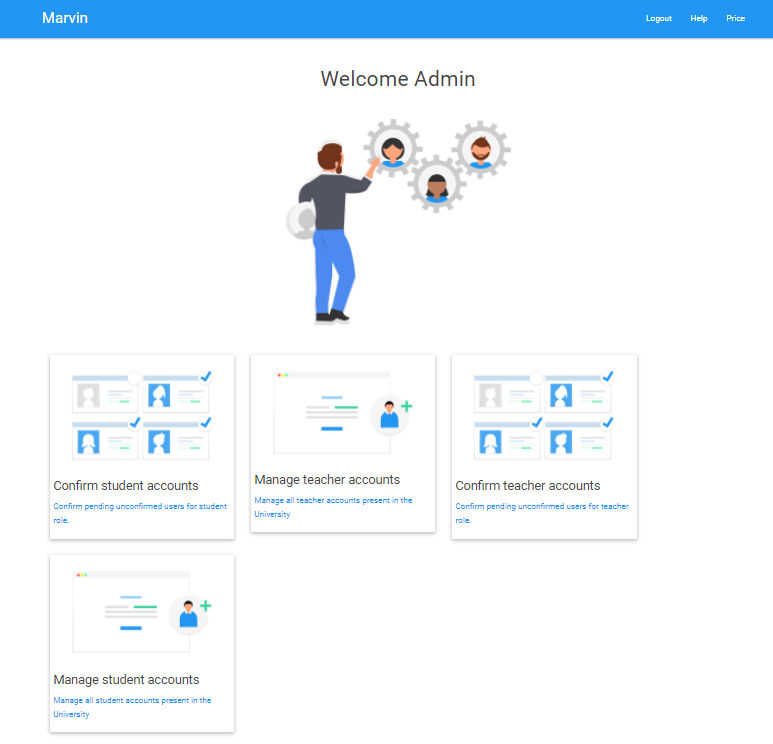
\includegraphics[width=1\linewidth]{image/Admin}
		\caption[Admin home page]{Admin home page}
		\label{fig:universityaddamin}
	\end{figure}
	
	\section{Students management}
	\subsection{Confirm or deny students accounts}
	\begin{enumerate}
		\item To open the page where you can confirm or deny pending students accounts, click on the \textquotedblleft Confirm students" link on the menu bar or the \textquotedblleft Confirm student accounts" link on the home page;
		\begin{figure}[H]
			\centering
			\fcolorbox{black}{white}{\includegraphics[width=0.8\linewidth]{"image/AdminConfStud1"}}
			\caption{Click on "Confirm students"}
			\label{fig:Click on "Confirm students"}
		\end{figure}
		\item Wait for the list to load;
		\item Click on the \textquotedblleft CONFIRM" button to confirm or on the \textquotedblleft DENY" button to deny the account on the desired student from the list.
		\begin{figure}[H]
			\centering
			\fcolorbox{black}{white}{\includegraphics[width=0.8\linewidth]{"image/AdminConfStud2"}}
			\caption{Click "CONFIRM"}
			\label{fig:Click "CONFIRM"}
		\end{figure}
	\end{enumerate}
	
	\subsection{Remove a student account}
	\begin{enumerate}
		\item Click on the \textquotedblleft Manage Users" link on the menu bar or on the home page;
		\begin{figure}[H]
			\centering
			\fcolorbox{black}{white}{\includegraphics[width=0.8\linewidth]{"image/AdminManageUser1"}}
			\caption{Click on "Manage Users"}
			\label{fig:Click on "Manage Users"}
		\end{figure}
		\item Wait for the list to load;
		\item Click on the \textquotedblleft DELETE" button to remove the desired student from the list.
		\begin{figure}[H]
			\centering
			\fcolorbox{black}{white}{\includegraphics[width=0.8\linewidth]{"image/AdminManageUser4S"}}
			\caption{Click "DELETE"}
			\label{fig:Click "DELETE"}
		\end{figure}
	\end{enumerate}
	
	\section{Teachers management}
	\subsection{Confirm or deny teachers accounts}
	\begin{enumerate}
		\item  To open the page where you can confirm or deny pending teachers accounts, click on the \textquotedblleft Confirm teacher" link on the menu bar or on the \textquotedblleft Confirm teacher accounts" link on the home page;
		\begin{figure}[H]
			\centering
			\fcolorbox{black}{white}{\includegraphics[width=0.8\linewidth]{"image/AdminConfTeach1"}}
			\caption{Click on "Confirm teacher"}
			\label{fig:Click on "Confirm teacher"}
		\end{figure}
		\item Wait for the list to load;
		\item Click on the \textquotedblleft CONFIRM" button to confirm or on the \textquotedblleft DENY" button to deny the account for the desired teacher from the list.
		\begin{figure}[H]
			\centering
			\fcolorbox{black}{white}{\includegraphics[width=0.8\linewidth]{"image/AdminConfTeach2"}}
			\caption{Click "CONFIRM"}
			\label{fig:Click "CONFIRM"}
		\end{figure}
	\end{enumerate}
	
	\subsection{Removeteachers accounts}
	\begin{enumerate}
		\item Click on the \textquotedblleft Manage Users" link on the menu bar or on the home page;
		\begin{figure}[H]
			\centering
			\fcolorbox{black}{white}{\includegraphics[width=0.8\linewidth]{"image/AdminManageUser1"}}
			\caption{Click on "Manage Users"}
			\label{fig:Click on "Manage Users"}
		\end{figure}
		\item Wait for the list to load;
		\item Click on the \textquotedblleft DELETE" button to remove the desired teacher from the list.
		\begin{figure}[H]
			\centering
			\fcolorbox{black}{white}{\includegraphics[width=0.8\linewidth]{"image/AdminManageUser2"}}
			\caption{Click "DELETE"}
			\label{fig:Click "DELETE"}
		\end{figure}
	\end{enumerate}
	
	
	\section{Courses management}
	\subsection{Add new courses}
	\begin{enumerate}
		\item Click on the \textquotedblleft Courses" link on the menu bar or on the \textquotedblleft Manage courses" link on the home page;
		\begin{figure}[H]
			\centering
			\fcolorbox{black}{white}{\includegraphics[width=0.8\linewidth]{"image/AdminManageCourses1"}}
			\caption{Click on "Courses"}
			\label{fig:Click on "Courses"}
		\end{figure} \newpage
		\item Fill the required fields;
		\begin{figure}[H]
			\centering
			\fcolorbox{black}{white}{\includegraphics[width=0.8\linewidth]{"image/AdminManageCourses2"}}
			\caption{Complete the required fields}
			\label{fig:Complete the required fields}
		\end{figure}
		\item Click on the \textquotedblleft SUBMIT" button.
		\begin{figure}[H]
			\centering
			\fcolorbox{black}{white}{\includegraphics[width=0.8\linewidth]{"image/AdminManageCourses3"}}
			\caption{Click "SUBMIT"}
			\label{fig:Click "SUBMIT"}
		\end{figure}
	\end{enumerate}
	\newpage
	\section{Exams management}
	\subsection{View the exams for an academic year}
	\begin{enumerate}
		\item Click on the \textquotedblleft Exams" link on the menu bar or on the home page;
		\begin{figure}[H]
			\centering
			\fcolorbox{black}{white}{\includegraphics[width=0.8\linewidth]{"image/adminExamYear1"}}
			\caption{Click on "Exams"}
			\label{fig:Click on "Exams"}
		\end{figure}
		\item Select the desired year to view all exams of that year.
		\begin{figure}[H]
			\centering
			\fcolorbox{black}{white}{\includegraphics[width=0.8\linewidth]{"image/adminExamYear2"}}
			\caption{Select the year}
			\label{fig:Select the year}
		\end{figure}
	\end{enumerate}
	\subsection{View the exams for a course}
	\begin{enumerate}
		\item Click on the \textquotedblleft Courses" link on the menu bar or on the \textquotedblleft Manage courses" link on the home page;
		\begin{figure}[H]
			\centering
			\fcolorbox{black}{white}{\includegraphics[width=0.8\linewidth]{"image/AdminManageCourses1"}}
			\caption{Click on "Courses"}
			\label{fig:Click on "Courses"}
		\end{figure}
		\item Wait for the course list to load;
		\item Click on the \textquotedblleft DETAILS" button of the desired course;
		\begin{figure}[H]
			\centering
			\fcolorbox{black}{white}{\includegraphics[width=0.8\linewidth]{"image/AdminManageCoursesExams1"}}
			\caption{Click on the course}
			\label{fig:Click on the course}
		\end{figure}
		\item Wait for the exam list to load.
		\begin{figure}[H]
			\centering
			\fcolorbox{black}{white}{\includegraphics[width=0.8\linewidth]{"image/AdminManageCoursesExams2"}}
			\caption{Wait for the exam list}
			\label{fig:Wait for the exam list}
		\end{figure}
	\end{enumerate}
	\newpage
	\subsection{Add new exams}
	\begin{enumerate}
		\item Click on the \textquotedblleft Courses" link on the menu bar or on the \textquotedblleft Manage courses" link on the home page;
		\begin{figure}[H]
			\centering
			\fcolorbox{black}{white}{\includegraphics[width=0.8\linewidth]{"image/AdminManageCourses1"}}
			\caption{Click on "Courses"}
			\label{fig:Click on "Courses"}
		\end{figure} \newpage
		\item Fill the required fields;
		\begin{figure}[H]
			\centering
			\fcolorbox{black}{white}{\includegraphics[width=0.8\linewidth]{"image/AdminNewExam1"}}
			\caption{Fill the required fields}
			\label{fig:Fill the required fields}
		\end{figure}
		\item And then click on the \textquotedblleft SUBMIT" button.
		\begin{figure}[H]
			\centering
			\fcolorbox{black}{white}{\includegraphics[width=0.8\linewidth]{"image/AdminNewExam2"}}
			\caption{Click "SUBMIT"}
			\label{fig:Click "SUBMIT"}
		\end{figure}
	\end{enumerate}
	\newpage
	\subsection{Associate teacher to an exam}
	\begin{enumerate}
		\item Click on the \textquotedblleft DETAILS" button next to the desired exam after \S 5.4.1 or \S 5.4.2;
		\begin{figure}[H]
			\centering
			\fcolorbox{black}{white}{\includegraphics[width=0.8\linewidth]{"image/AdminAssociateTeach1"}}
			\caption{Click on "DETAILS"}
			\label{fig:Click on "DETAILS"}
		\end{figure}
		\item Click on the \textquotedblleft ASSIGN TEACHER" button to assign a teacher to the selected exam;
		\begin{figure}[H]
			\centering
			\fcolorbox{black}{white}{\includegraphics[width=0.8\linewidth]{"image/AdminAssociateTeach2"}}
			\caption{Click on "ASSIGN TEACHER"}
			\label{fig:Click on "ASSIGN TEACHER"}
		\end{figure}
		\item Select the desired teacher and then click on the \textquotedblleft YES" button to confirm;
		\begin{figure}[H]
			\centering
			\fcolorbox{black}{white}{\includegraphics[width=0.8\linewidth]{"image/AdminAssociateTeach3"}}
			\caption{Click "YES" after selecting the teacher}
			\label{fig:Click "YES" after selecting the teacher}
		\end{figure}
	\end{enumerate}
	
\end{document}